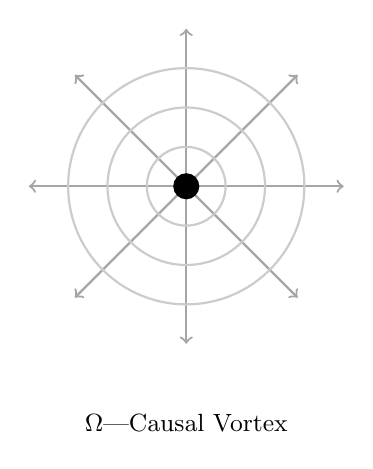
\begin{tikzpicture}[
    vec/.style={->, thick, draw=gray!70}
]

\foreach \a in {0,45,...,315}{
   \draw[vec] (0,0) -- ++({2*cos(\a)},{2*sin(\a)});
}

\foreach \r in {0.5,1,1.5}{
  \draw[gray!40, thick] (0,0) circle (\r);
}

\node[circle,fill=black,minimum size=7pt] at (0,0) {};

\node at (0,-3) {\small $\Omega$---Causal Vortex};

\end{tikzpicture}